% Déclaration du type de document (report, book, paper, etc...)
\documentclass[a4paper]{paper} 
 
% Package pour avoir Latex en français
\usepackage[utf8]{inputenc}
\usepackage[T1]{fontenc}
\usepackage[frenchb]{babel}
 
% Quelques packages utiles
\usepackage{listings} % Pour afficher des listings de programmes
\usepackage{graphicx} % Pour afficher des figures
\usepackage{amsthm}   % Pour créer des théorèmes et des définitions
\usepackage{amsmath}
\usepackage{microtype} % Optical margins FTW
\usepackage{url}
\usepackage{booktabs} % Allows the use of \toprule, \midrule and \bottomrule in tables for horizontal lines
\usepackage[per-mode=symbol]{siunitx}
\usepackage{floatrow}
\usepackage{caption}
\usepackage{subcaption}
\usepackage{mhchem}

\title{Estimations des coûts}
\author{Antoine Albertelli \and Quentin Herzig}

% Unités customs pour les francs et les pièces
\DeclareSIUnit\chf{\textsc{chf}}
\DeclareSIUnit\piece{pièce}
\DeclareSIUnit\annee{année}
\DeclareSIUnit\an{an}



% Début du document
\begin{document}
\maketitle

\begin{table}[h!]
\centering 
\begin{tabular}{l S[table-format=3.2] r} 
\toprule 
\multicolumn{2}{l}{\textbf{Électricité}} & \\ 
Consommation électrique & 5 & \si{\kilo\watt} \\
Prix de l'électricité & 0.2 & \si{\chf\per\kilo\watt\per\hour} \\
\cmidrule(l){2-3}
Coût d'électricité & 1 & \si{\chf\per\hour} \\
\midrule
\multicolumn{2}{l}{\textbf{Machines}} & \\ 
Presse électrique & 130000 & \si{\chf} \\
Fonctionnement & 6240 & \si{\hour\per\annee} \\
\cmidrule(l){2-3}
Amortissement sur 5 ans & 4.17 & \si{\chf\per\hour} \\
\midrule
\multicolumn{2}{l}{\textbf{Opérateurs}} & \\ 
Opérateur à 10\% & 6& \si{\chf\per\hour} \\
\midrule

\multicolumn{2}{l}{\textbf{Matière}} & \\ 
Matière (\textsc{pc}) & 11 & \si{\chf\per\kilogram} \\ 
Poids de la pièce & 25 & \si{\gram} \\
\cmidrule(l){2-3}
Coût de la matière & 0.27 & \si{\chf\per\piece} \\

\midrule
\multicolumn{2}{l}{\textbf{Outillage}} & \\ 
Prix du moule & 20000 & \si{\chf} \\
Pièces par série & 20000& \si{\piece} \\
\cmidrule(l){2-3}
Coûts d'outillage & 1 & \si{\chf\per\piece} \\

\midrule
\midrule
Coût horaire & 11.67  & \si{\chf\per\hour} \\
Temps de cycle & 20 & \si{\second\per\piece} \\
\cmidrule(l){2-3}
\textbf{\textsc{Total}} & 1.34 & \si{\chf\per\piece} \\

\bottomrule 
\end{tabular}
\caption{Calcul des coûts de l'injection plastique} 
\label{tab:cost-molding}
\end{table}



\begin{table}[h!]
\centering 
\begin{tabular}{l S[table-format=3.2] r} 
\toprule 
\multicolumn{2}{l}{\textbf{Électricité}} & \\ 
Consommation électrique & 2.5 & \si{\kilo\watt} \\
Prix de l'électricité & 0.2 & \si{\chf\per\kilo\watt\per\hour} \\
\cmidrule(l){2-3}
Prix de l'électricité & 0.5 & \si{\chf\per\hour} \\
\midrule
\multicolumn{2}{l}{\textbf{Machines}} & \\ 
LPKF Microline 160i & 220000 & \si{\chf} \\
Fonctionnement & 6240 & \si{\hour\per\annee} \\
\cmidrule(l){2-3}
Amortissement sur 5 ans& 7.05 & \si{\chf\per\hour} \\
\midrule
\multicolumn{2}{l}{\textbf{Opérateurs}} & \\ 
Opérateur à 100\% & 60& \si{\chf\per\hour} \\

\midrule
\multicolumn{2}{l}{\textbf{Temps de cycle}} & \\ 
Vitesse du laser & 4000 & \si{\milli\meter\per\second} \\
Diamètre du laser & 80 & \si{\micro\meter} \\
Vitesse de balayage & 320 & \si{\milli\meter\squared\per\second} \\
Surface des pistes & 1800 & \si{\milli\meter\squared\per\piece} \\ 
Temps de balayage & 5.625 & \si{\second\per\piece} \\ 
Temps de positionnement & 1 & \si{\second\per orientation} \\
Nombre d'orientations & 5 &  \\
Temps de mise en place, retrait et inspection & 15 & \si{\second\per\piece} \\ 

\cmidrule(l){2-3}
\textbf{Temps total} & 25.625 & \si{\second\per\piece} \\ 

\midrule
\midrule
Coût horaire & 67.68 & \si{\chf\per\hour} \\
Temps de cycle & 25.625 & \si{\second\per\piece} \\
\cmidrule(l){2-3}
\textbf{\textsc{Total}} & 0.48 & \si{\chf\per\piece} \\

\bottomrule 
\end{tabular}
\caption{Calcul des coûts de l'activation sélective par laser} 
\label{tab:cost-laser-activation}
\end{table}

\begin{figure}[h]
    \begin{center}
        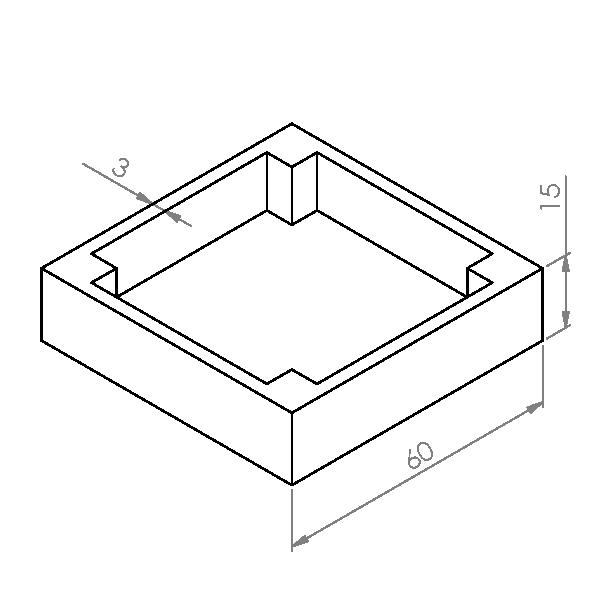
\includegraphics[width=0.6\textwidth]{images/example_part/example_mid}
        \caption{Pièce d'exemple. Les dimensions et la géométrie sont approximatives.}\label{fig:example-part}
    \end{center}
\end{figure}

\end{document}
